\documentclass{beamer}
\usepackage[utf8]{inputenc}
\usetheme{Singapore}
\usecolortheme{default}
\usepackage{graphicx}
\beamertemplatenavigationsymbolsempty


\title[Genetic algorithm for QSVM] 
{Genetic algorithm for Quantum Support Vector Machines}

\author[Lorenzo Tasca]
{Lorenzo Tasca}
 
\institute[]
{

  Dipartimento di Fisica “Giuseppe Occhialini”\\
  Università degli Studi di Milano-Bicocca\\\,\\
  Relatore: Alberto Ottavio Leporati\\
  Correlatore: Alberto Zaffaroni
  
}
\date[25/11/2024] 
{25 Novembre 2024}

\logo{
\includegraphics[height=1cm]{images/logo.png}}

\begin{document}

\frame{\titlepage}

\begin{frame}
\frametitle{Quantum Machine Learning  +  Genetic Algorithm}
\centering
     \begin{minipage}{0.5\textwidth}
      \centering
      
\includegraphics[width=\textwidth]{images/1.png}
  \end{minipage}%
  \begin{minipage}{0.5\textwidth}
      \centering
      
\includegraphics[width=0.8\textwidth]{images/genetic-algorithms-in-python.png}
  \end{minipage}
\end{frame}



\begin{frame}
  \frametitle{Support Vector Machine}
    \begin{itemize}
      \item La SVM è un algoritmo supervisionato di classificazione binaria.
    \end{itemize}
      \begin{figure}
            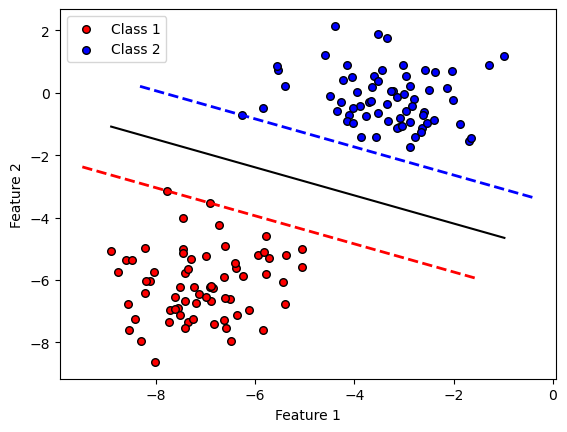
\includegraphics[width=0.7\textwidth]{images/classicalsvm.png}
       \end{figure}
  \end{frame}

  \begin{frame}
    \frametitle{Kernel Support Vector Machine}
    \begin{columns}
      \column{0.5\textwidth}
    
      \begin{itemize}
        \item Nel caso in cui i dati non siano linearmente separabili?\\\,
        \item È possibile applicare una feature map $\phi(\mathbf{x})$.\\\,
        \item $K_{ij}=\langle \phi(\mathbf{x}_i), \phi(\mathbf{x}_j)\rangle$. \\\,\\\,
      \end{itemize}
      
      \column{0.5\textwidth}
   
  
      \begin{minipage}{\textwidth}
        \centering
        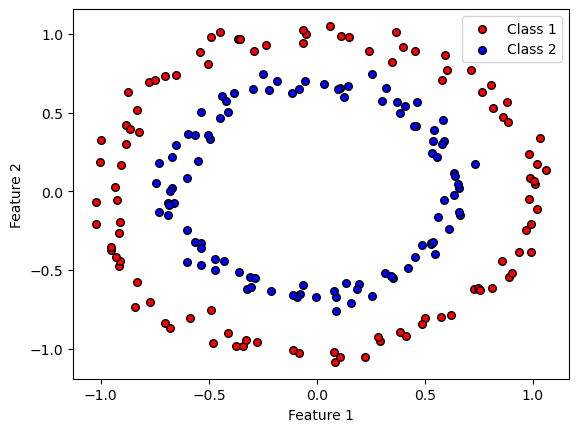
\includegraphics[width=0.8\textwidth]{images/circles.png}
    \end{minipage}
    \begin{minipage}{\textwidth}
        \centering
        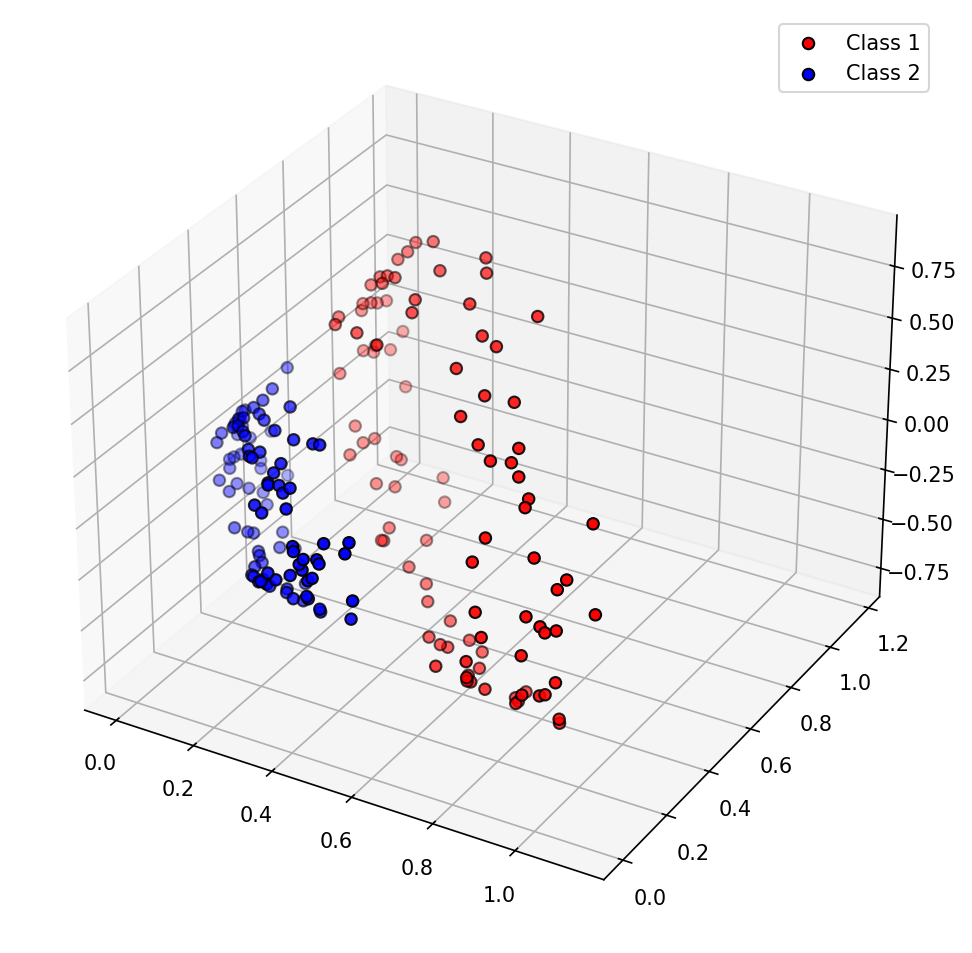
\includegraphics[width=0.8\textwidth]{images/circles3d.png}
    \end{minipage}
  
      
      \end{columns}
  
  \end{frame}




\begin{frame}
  \frametitle{Quantum Support Vector Machine}
  \begin{columns}
    \column{0.5\textwidth}
  
    \begin{itemize}
      \item La feature map diventa un circuito quantistico parametrizzato. \\\,
          \item $|\phi(\mathbf{x})\rangle=U(\mathbf{x})|0\rangle^{\otimes n}$.\\\,
          \item$K_{ij}=\langle \phi(\mathbf{x}_i)| \phi(\mathbf{x}_j) \rangle.$\\\,\\\,
          \end{itemize}
    
    \column{0.5\textwidth}
    \begin{figure}
          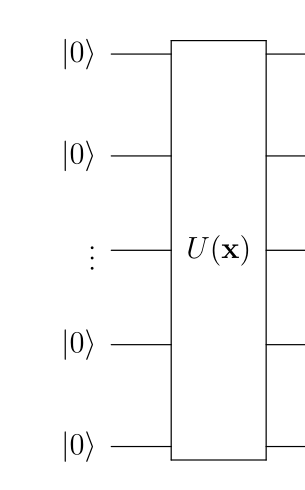
\includegraphics[width=0.7\textwidth]{images/Pasted image.png}
     \end{figure}


    
    \end{columns}

\end{frame}


\begin{frame}
  \frametitle{Quantum Kernels}
  
  \begin{itemize}
    \item Un esempio: la ZZ Feature Map.
    \item  Ottime performance su dataset complessi.  
  \end{itemize}
     
\vspace{0.8cm}
       \begin{minipage}{0.5\textwidth}
          \centering
          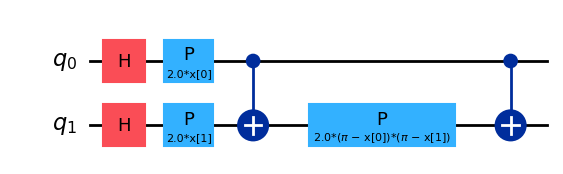
\includegraphics[width=\textwidth]{images/ZZ.png}
      \end{minipage}%
      \begin{minipage}{0.5\textwidth}
          \centering
          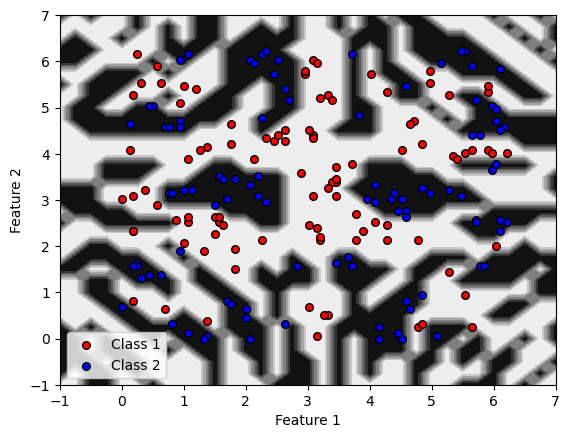
\includegraphics[width=\textwidth]{images/adhoczz.png}
      \end{minipage}
        
\end{frame}

\begin{frame}
  \frametitle{Quantum Kernels}
  \begin{itemize}
    \item I metodi classici falliscono.
  \end{itemize}
    \vspace{0.8cm}
    \begin{minipage}{0.5\textwidth}
       \centering
       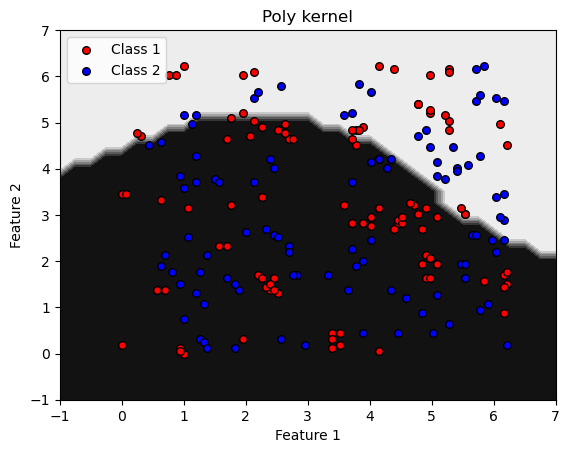
\includegraphics[width=\textwidth]{images/adhocpoly.png}
   \end{minipage}%
   \begin{minipage}{0.5\textwidth}
       \centering
       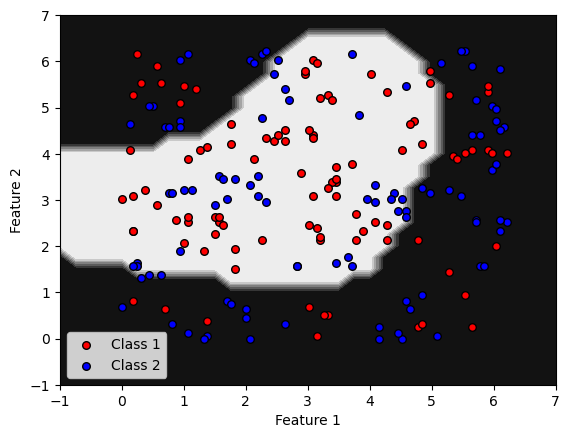
\includegraphics[width=\textwidth]{images/adhocrbf.png}
   \end{minipage}
\end{frame}


\begin{frame}
  \frametitle{Quantum Kernel}
  \begin{itemize}
    \item Tuttavia la scelta del kernel risulta spesso problematica. 
  \end{itemize}
  \vspace{0.8cm}
  \begin{minipage}{0.5\textwidth}
     \centering
     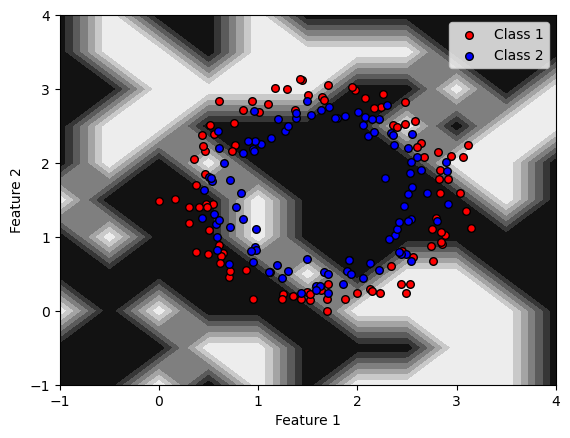
\includegraphics[width=\textwidth]{images/failcircle.png}
 \end{minipage}%
 \begin{minipage}{0.5\textwidth}
     \centering
     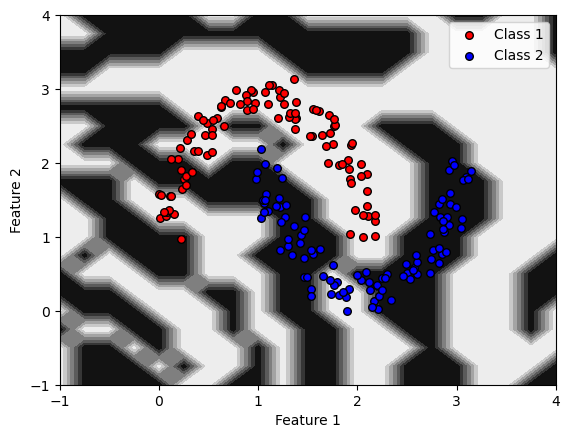
\includegraphics[width=\textwidth]{images/failmoon.png}
 \end{minipage}
\end{frame}

\begin{frame}
  \frametitle{Genetic algorithm}
  \begin{itemize}
    \item Un algoritmo genetico può scegliere la miglior feature map.\\\,
  \end{itemize}

  \begin{figure}
    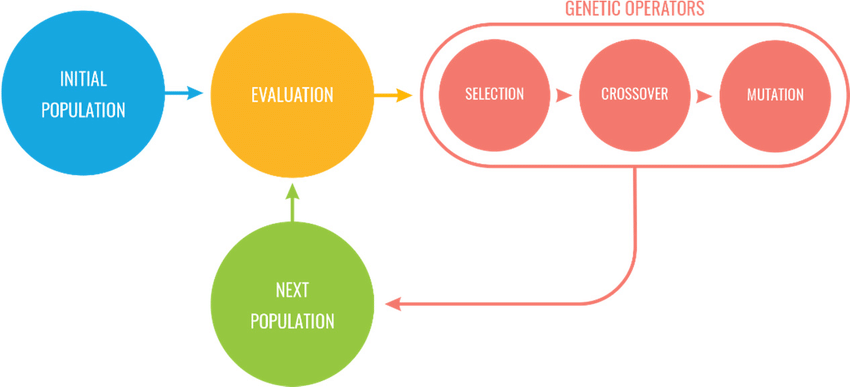
\includegraphics[width=\textwidth]{images/genetic.png}
  \end{figure} 
\end{frame}


\begin{frame}
  \frametitle{Genetic algorithm}
  \begin{itemize}
    \item Gli individui sono formati da gate scelti da un set completo.
    \item La prima generazione è generata in maniera casuale. 
  \end{itemize}
  \vspace{0.5cm}
  \begin{minipage}{0.5\textwidth}
    \centering
    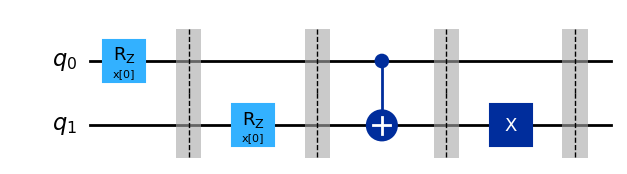
\includegraphics[width=\textwidth]{images/fenotip.png}
\end{minipage}%
\begin{minipage}{0.5\textwidth}
    \centering
    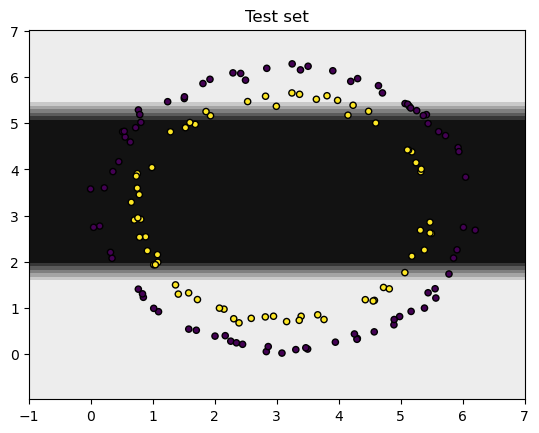
\includegraphics[width=\textwidth]{images/badresult.png}
\end{minipage}
\end{frame}

\begin{frame}
  \frametitle{Genetic algorithm}
  \begin{itemize}
    \item La fitness di un individuo si calcola a partire dalla sua accuratezza.
    \item Gli individui sono passati alla seguente generazione con il crossover.
    \vspace{0.5cm}

  \centering \textit{Parent individuals}    \,\,\,\,\,\,\,
  \end{itemize}
  \begin{minipage}{0.5\textwidth}
    \centering
    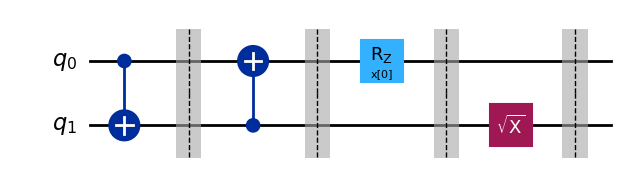
\includegraphics[width=\textwidth]{images/parent1.png}
\end{minipage}%
\begin{minipage}{0.5\textwidth}
    \centering
    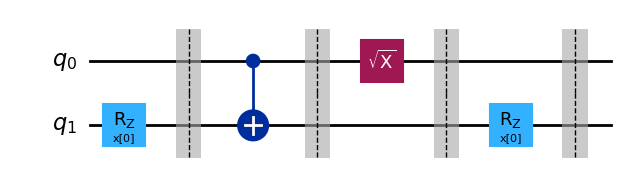
\includegraphics[width=\textwidth]{images/parent2.png}
\end{minipage}

\vspace{0.5cm}
\centering \textit{Child individuals}
\begin{minipage}{0.5\textwidth}
    \centering
    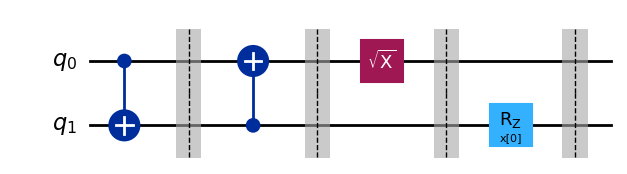
\includegraphics[width=\textwidth]{images/child1.png}
\end{minipage}%
\begin{minipage}{0.5\textwidth}
    \centering
    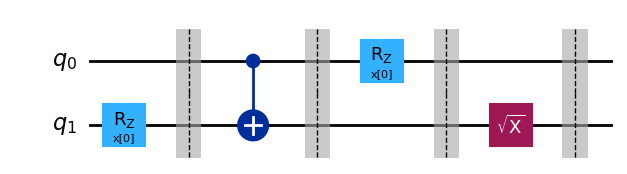
\includegraphics[width=\textwidth]{images/child2.png}
\end{minipage}

\end{frame}


\begin{frame}
  \frametitle{Genetic algorithm}
  \begin{itemize}
    \item Inoltre subiscono una mutazione casuale.  
  \end{itemize}

  \begin{figure}
    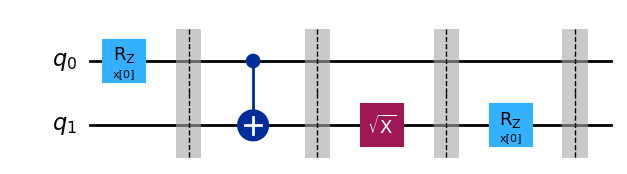
\includegraphics[width=0.9\textwidth]{images/nonmutated.png}
  \end{figure} 
  \begin{figure}
    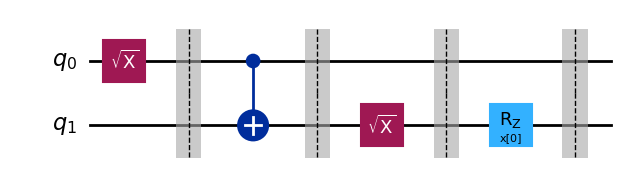
\includegraphics[width=0.9\textwidth]{images/mutated.png}
  \end{figure} 
\end{frame}

\begin{frame}
  \frametitle{Genetic algorithm}
  \begin{itemize}
    \item Con l'andare delle generazioni aumenta l'accuratezza media e quella massima.
  \end{itemize}
  \vspace{0.8cm}

  \begin{minipage}{0.5\textwidth}
    \centering
    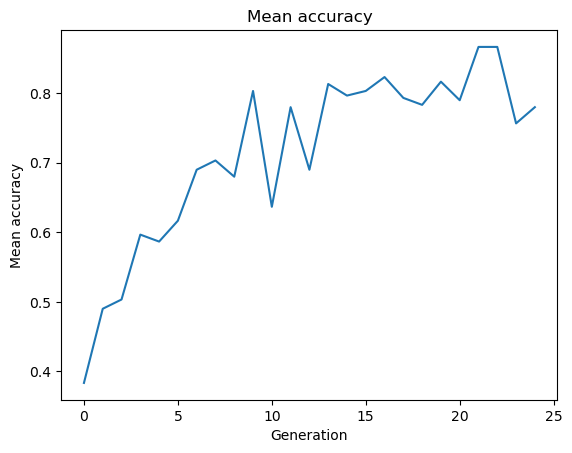
\includegraphics[width=\textwidth]{images/meanaccuracy.png}
\end{minipage}%
\begin{minipage}{0.5\textwidth}
    \centering
    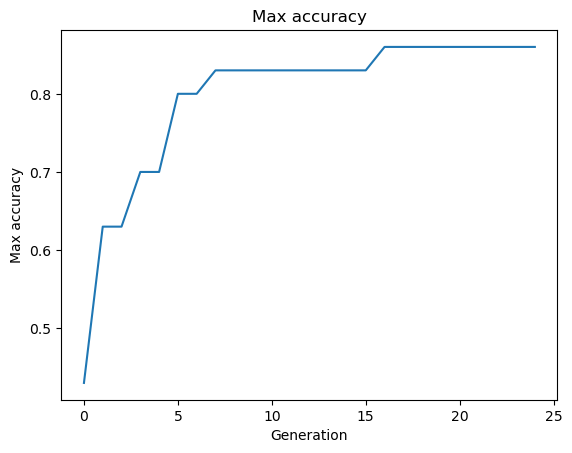
\includegraphics[width=\textwidth]{images/maxaccuracy.png}
\end{minipage}
\end{frame}


\begin{frame}
  \frametitle{Genetic algorithm}
  \begin{itemize}
    \item Otteniamo così un circuito ad alte prestazioni, impossibile da ottenere manualmente.
  \end{itemize}
  \vspace{0.8cm}

  \begin{minipage}{0.5\textwidth}
    \centering
    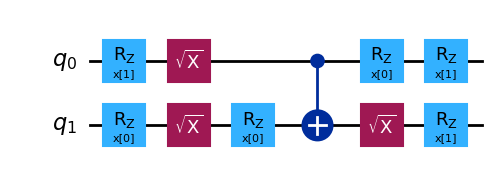
\includegraphics[width=\textwidth]{images/finalcircuit.png}
\end{minipage}%
\begin{minipage}{0.5\textwidth}
    \centering
    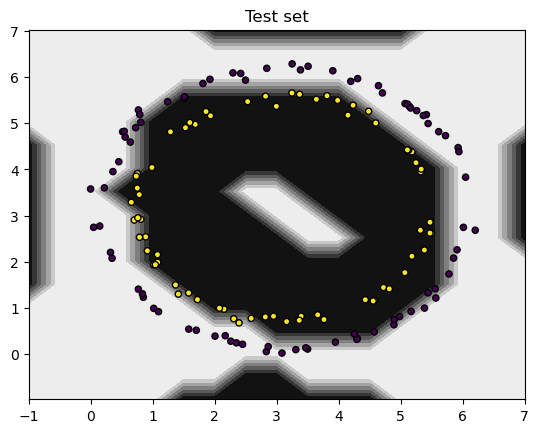
\includegraphics[width=\textwidth]{images/awesomeresult.png}
\end{minipage}
\end{frame}


\begin{frame}
  \frametitle{Genetic algorithm}
  \begin{itemize}
    \item L'algoritmo si dimostra robusto al rumore e a variazioni della forma dei dati.
  \end{itemize}
  \vspace{0.8cm}

  \begin{minipage}{0.5\textwidth}
    \centering
    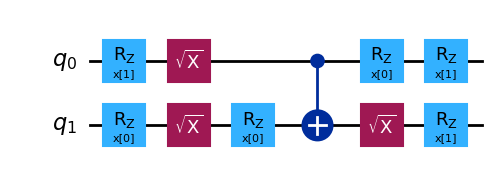
\includegraphics[width=\textwidth]{images/finalcircuit.png}
\end{minipage}%
\begin{minipage}{0.5\textwidth}
    \centering
    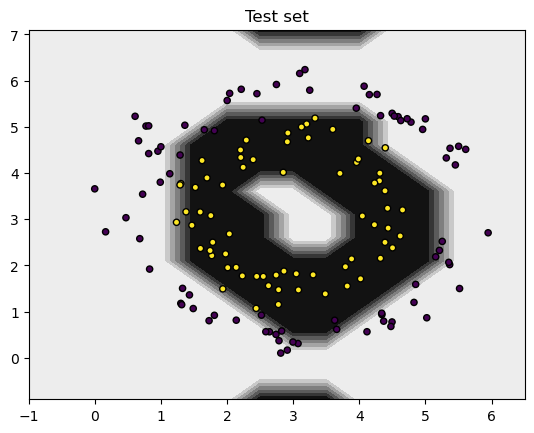
\includegraphics[width=\textwidth]{images/noise.png}
\end{minipage}
\end{frame}

\begin{frame}
  \frametitle{Genetic algorithm}
  \begin{itemize}
    \item L'algoritmo si dimostra funzionante su vari tipi di dataset, sia artificiali che reali. 
  \end{itemize}
  \vspace{0.8cm}

  \begin{minipage}{0.5\textwidth}
    \centering
    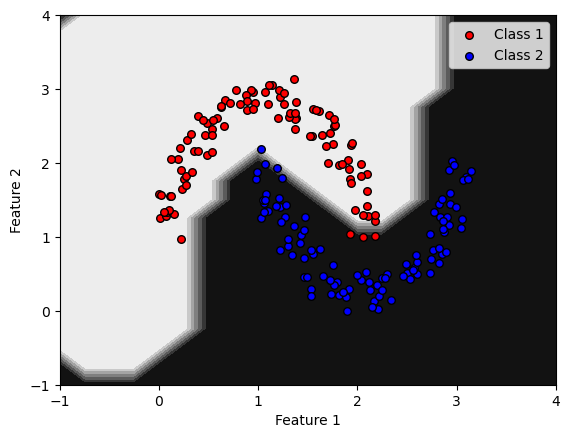
\includegraphics[width=\textwidth]{images/moonsrbf.png}
\end{minipage}%
\begin{minipage}{0.5\textwidth}
    \centering
    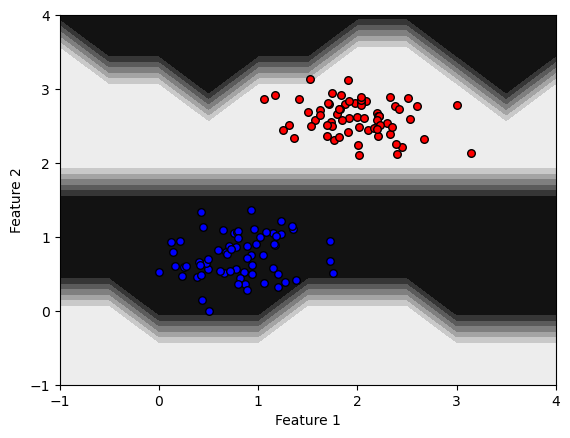
\includegraphics[width=\textwidth]{images/qsvm.png}
\end{minipage}
\end{frame}

\begin{frame}
  \frametitle{Directions for Future Work?}
  \begin{itemize}
    \item L'algoritmo andrebbe ora testato su dataset multidimensionali, e infine su un reale dispositivo quantistico scalabile.
  \end{itemize}
  \vspace{0.8cm}

  \begin{minipage}{0.5\textwidth}
    \centering
    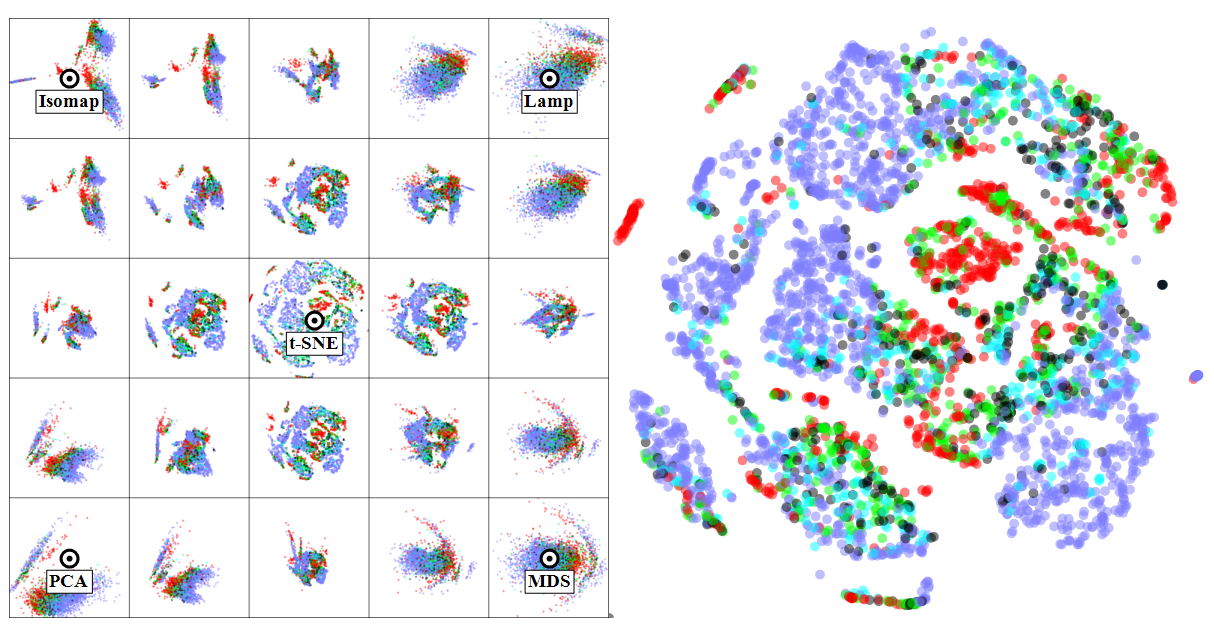
\includegraphics[width=\textwidth]{images/multi.png}
\end{minipage}%
\begin{minipage}{0.5\textwidth}
    \centering
    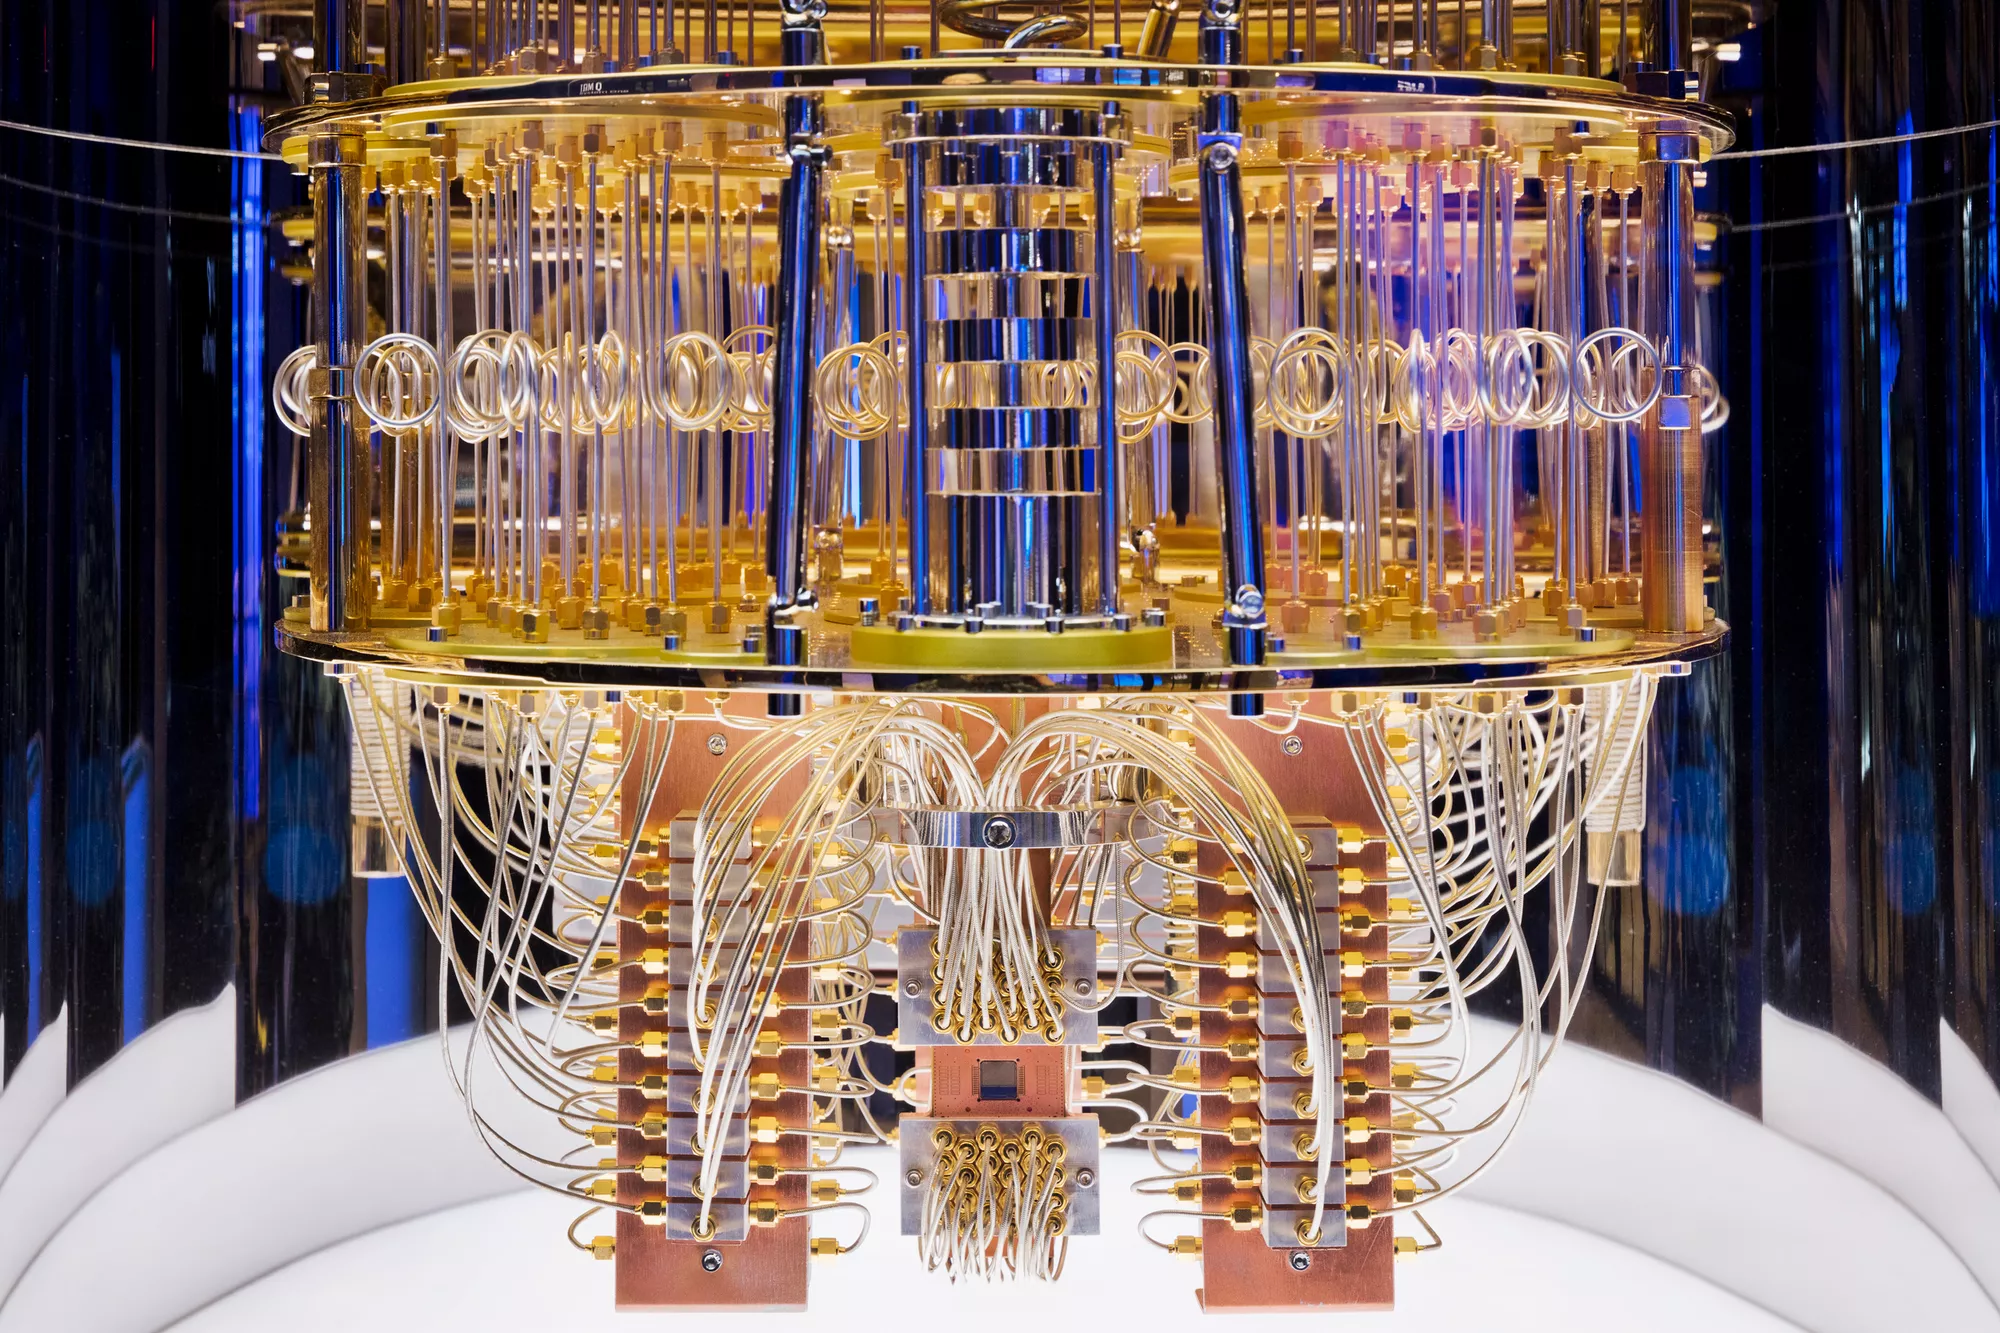
\includegraphics[width=\textwidth]{images/device.png}
\end{minipage}
\end{frame}

\begin{frame}
\centering Grazie per l'attenzione!

\end{frame}

\end{document}